%! Author = trevo
%! Date = 4/18/2024

% Preamble
\documentclass[12pt]{report}

% Packages
\usepackage{amsmath,geometry,setspace, enumerate,pdfpages}
\usepackage{hyperref}
\usepackage[british]{babel}
\usepackage{csquotes}
\usepackage[round]{natbib}
\bibliographystyle{plainnat}
\doublespacing
\setlength\parindent{24pt}

\begin{document}
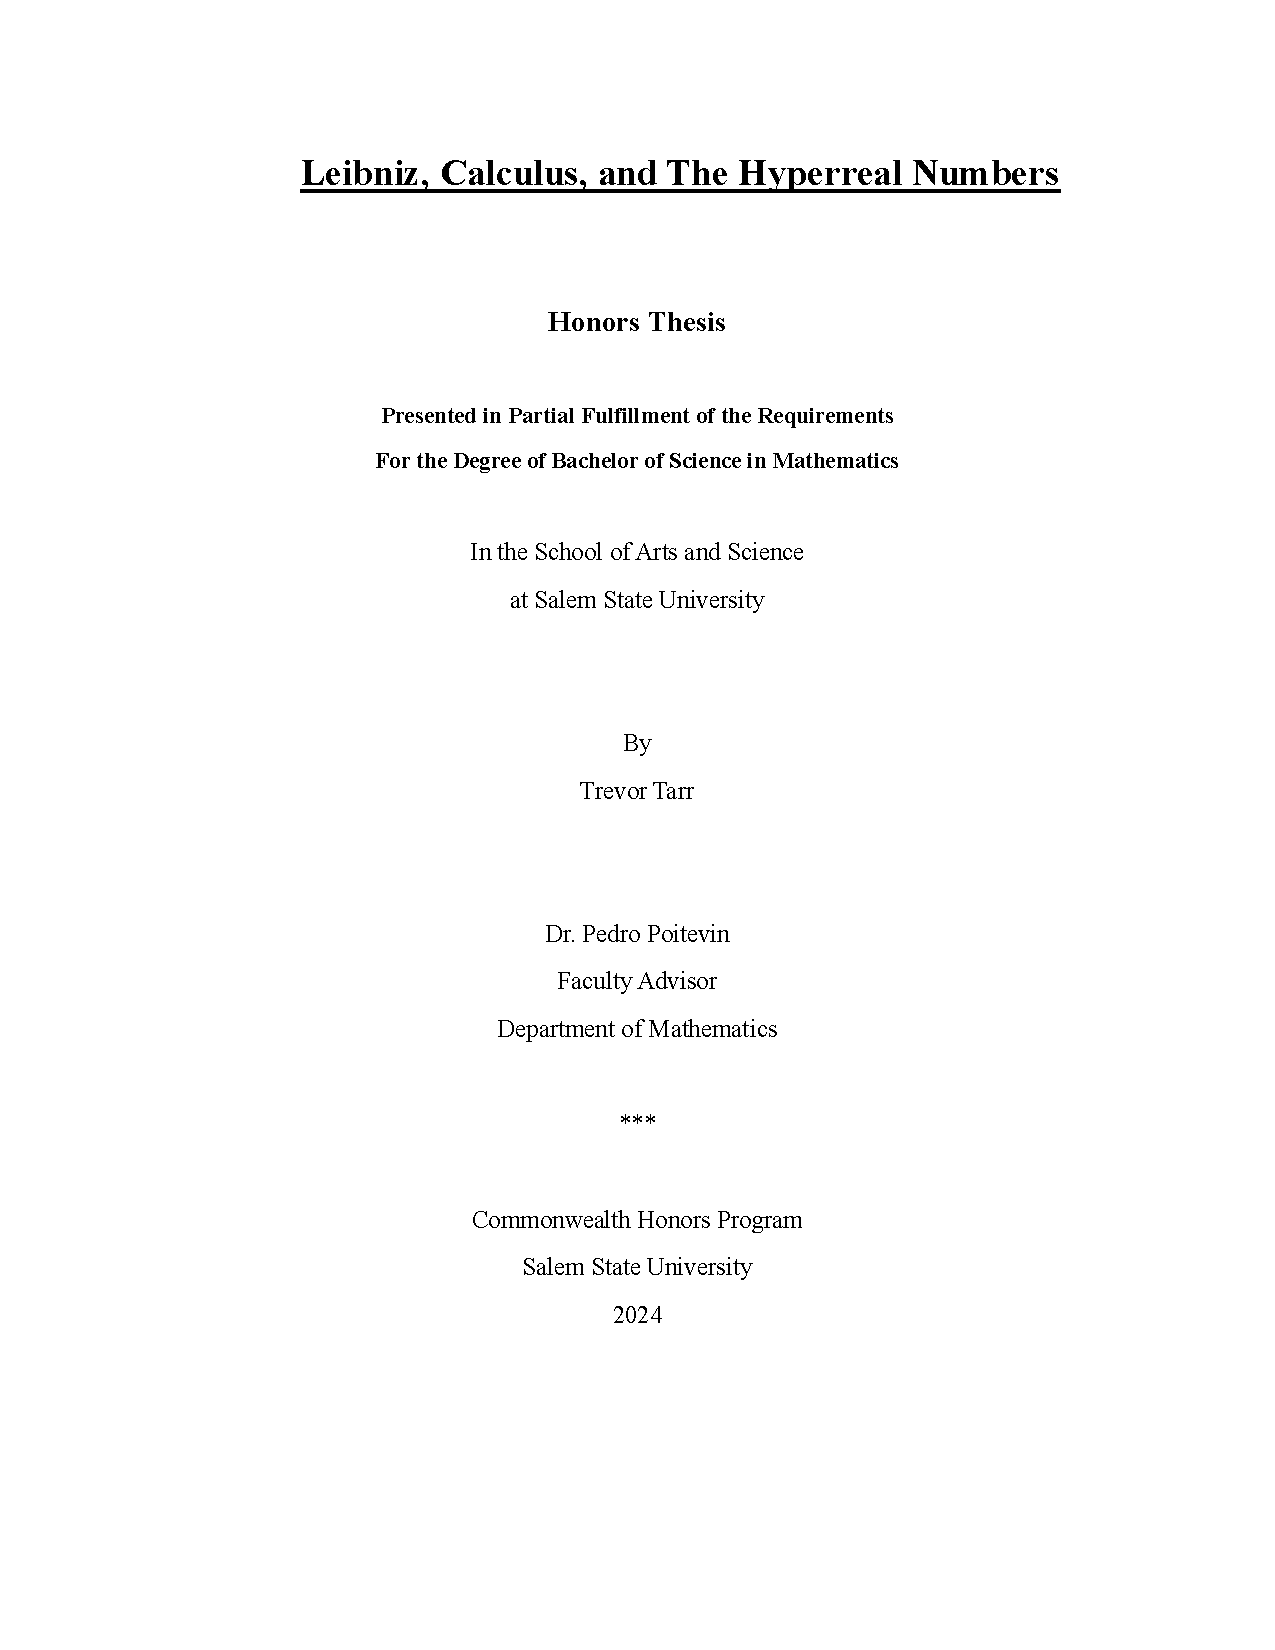
\includepdf[pages=1]{title}
    \newpage
\pagenumbering{gobble}
    \newpage
    \pagenumbering{roman}



\section*{\underline{Abstract}}
Our ideas revolving around Calculus, Philosophy, Law, and Theology are often so clouded that we forget to acknowledge the people behind these ideas.
We are taught these ideas within near hours, days, or as much as months and yet only scratch the surface.
Through this way of thinking, we forget to look at the foundations that took countless years and even lifetimes to construct out of what we believe to be nothingness.
What if I were to say everything mentioned in the first sentence was revolutionized by a German mathematician, philosopher, and logician's name is Gottfried Wilhelm Leibniz(\citauthor{Belaval}).
The first part of this paper will focus on outlining his contributions to the foundations and invention of Calculus, disagreements between him and Newton regarding Calculus, Leibniz's notation for Calculus, and some of his other work in other areas such as law, metaphysics, and much more.
The second part of this paper will focus on Abraham Robertson's construction of the Hyperreal Numbers and their applications proving that Leibniz's intuition of infinitesimals and Calculus correct.
This paper will not cover personal aspects, including his personal life (birth, death, spouses, etc.) as that does not align with the goal of this paper.
Accurate recognition of one's work is critical in maintaining not only credibility over future pieces of work but also recognizing the accomplishments of one's work.
Understanding Leibniz's work and the instrumental construction of Calculus and infinitesimals allows us to also focus on the foundations of our modern societies and trace where many of our common ideas and innovations stem from.
Ultimately, by the end of this paper, one should have a better understanding of the impact Leibniz, infinitesimals, and the foundational understandings of Calculus.
\newpage
\section*{\textit{Acknowledgements}}
\begin{itshape}
    Firstly, I'd like to thank Gottfried Wilhelm Leibniz himself for his dedication to academia, which expanded our understanding of various structures of society and reason.\newline \newline
    I am extremely grateful for my professor and advisor Dr.Pedro Poitevin, who not only advised me and took time with me to form this work but also educated me in standard and non-standard analysis.\newline\newline
    I would also like to thank Dr.Jeff Theis for working with me to edit and ensure the structure of the work was up to standards.\newline \newline
    Importantly, I want to express my deepest appreciation for the support from my family, including my Mother, Aunt, Grandmother, and others.
    Without them, I would not have had the support and resources to mentally and physically write, study and research this and many other topics simultaneously.
\end{itshape}
\newpage
\pagenumbering{arabic}
\part{Leibniz's Work}
\newpage

\chapter{Infinitesimals}

    \section*{Context}
Leibniz theorized that numbers existed that were infinitely small and/or infinitely great referred to as infinitesimal numbers.
Focused on this idea, Leibniz utilized this idea of infinitesimals to conceptualize the changes in small quantities that led to the idea of the derivative in Calculus (\citauthor{Goldblatt}, 11).
Calculus to Leibniz was the examination and manipulation of infinitesimal values.
While his ideas about infinitesimals were often challenged during his time by many, including Issac Newton, ultimately with the mind of Abraham Robinson in the 1960s, his ideas were ultimately proven to not only exist but also be the fundamental ideas behind calculus, especially when it comes to the derivative and the integral.

\section*{Metaphysical and Theological Perspective}
Leibniz pondered the question on how we live in the most perfect of possible universes.
The idea follows that given some of what he referred to as 'substances' in a non-contradictory combination of existing substances comprise a possible universe in Christian Creationism.
For example, we will use $l, m, n, o, p$ as our substances.
Let's per se we add the following condition onto our substances:
    \begin{enumerate}
        \item Substance $l$ cannot coexist with substance $m$.
        \item Substance $o$ can only coexist with substances $l \ \& \ n$.
    \end{enumerate}
The goal of creation for God, according to Leibniz, is to create a universe with the most substance (most perfect) (\citauthor{Strickland}, 29-31). \\
By this we could get a set containing all the possible.
Some elements can coexist together while some can't.
By creating such a collection of filters, the maximal element of such a filter would be the maximal filter that as such would yield the most perfect universe.
While with four substances it is straightforward, with an unknown amount(most likely infinite) on a grander scale, we can find such a filter used to derive the most perfect universe, which by Leibniz's reasoning on God's perfection in creation, is our universe.
This idea of a maximal element, maximum filter and filters would be where we start to set the scene for the roots of Calculus.

    \section*{The Hyperreal numbers and Continuity}
In 1966, these ideas about maximum filters and infinitesimals are what led mathematician Abraham Robinson to lay out the foundations of what we know today are the Hyperreal number system.
The Hyperreal numbers are an extension of the Real numbers symbolized as infinite sequences of Real numbers (\citauthor{Goldblatt},30-33).
This extension of the real number system allows us to understand continuity and differentiation in calculus the same way as Leibniz had developed roughly 300 years prior.
If two infinitesimals are infinitely close to each other (i.e. $ x \approx c$) then through a function($f$):  $f(x) \approx  f(c)$, (\citauthor{Goldbring}, 81-82).
From here we can say that through the points the function is continuous.
We know that derivative exists for any continuous function in its domain.
Thus, this will bring us into Leibniz's work with derivatives.

    \section*{The Derivative}
To Leibniz, the $dx$ symbol (or with any other letter instead of $x$) symbolized the differential with respect to a variable (or multiple).
Ultimately, the derivative symbolized changes in infinitesimal values based on the slope of the tangent line, as Leibniz has originally proposed (\citauthor{Goldblatt}, 5).
What one is taught is that for finding the derivative is: \[\frac{d}{dx} = \lim_{h \xrightarrow{} \infty} \frac{f(x+h)-f(x)}{h}\] While we are taught that x and h are real numbers, Leibniz proposed that they are what we know as now as hyperreal numbers (as we know of the now) and thus $\frac{dy}{dx}$  is a quotient of infinitesimals describing infinitesimal differences of rate of change.
This idea, while not initially accepted, ultimately was shown to be the foundational idea behind the inner workings of differential calculus.\\ \par
    One way of manipulating derivatives derived by Leibniz is what we know as the Product Rule.
The Product Rule (or Leibniz's Rule) is a method of taking the derivative of two functions that are multiplied. (\citauthor{Leibniz}, 2).
Given two variables $x \ \& \  y$, the derivative of the product is the sum of $x$ multiplied by the derivative of $y$ and $y$ multiplied by the derivative of $x$. As a formula:  $dxy=xdy+ydx$ .

    \section*{The Integral}
Like Riemann Sums, Leibniz idealized that finding the area under any graph starts with finding the area of infinite many polygons under that graph across an infinitesimal interval. 
The $\int$ symbol was Leibniz's notation for integrals derived from the word "Sum" (in Latin: "Summa"). 
This proposition was in conjunction with another credited contributor of what we know as "Integration," Johann Bernoulli. 
Bernoulli originally proposed using a capital "$I$" to denote integration, but to Leibniz's suggestion $\int$ become then deciding symbol as "$I$" closely resembled many other symbols in mathematics (\citauthor{Cajori},412-413).
This would prove to be an insightful suggestion as today many other symbols use Greek and Latin capital lettering and thus would diminish the impact and prevalence of the meaning of integration with a definition like "I". It can also be universally accepted without the knowledge of other languages or confusion with other languages and in programming.  
The use of $dx$ at the end came as a symbol to denote which differential variable was being integrated on.
    
    \section*{The Rivalry of Leibniz and Newton}
Between 1665 and 1666, Sir Issac Newton first laid out and made known in his work his methods on fluxions.
Newton's ideas revolve around change regarding the passage of time.
His published work known as "\textit{De Analysi}" included his work on these new methods.
Independently, Leibniz developed his ideas in 1675.
His methods focused on the infinitesimal changes of the slope of a general graph (unlike Newton who specifically mentions time as an axis.). While Newton was the first development, Leibniz was the first to publish his work in the mid-1680s through newspaper articles (\citauthor{Bardi}, $v$). \par
While at first acknowledging each other's accomplishments through letter communications, Newton grew ever so paranoid over Leibniz's discoveries.
It had been known that Leibniz had previously looked at Newton's work through a connection and the Royal Society and had taken notes.
Records indicate that these notes we rent used in any manner to claim Newtons work as one's own (\citauthor{Bardi}, 96).
Leibniz proposed an approach to Calculus steered away from Newtons in many aspects.
While Newton mainly stayed on physical-based assumptions and relations to time, Leibniz took the approach to generalize it and focus on the infinitesimals at play.
Newton's paranoia only grew worse as at the same time, Robert Hooke was laying claim to Newton's discoveries laid out in works including "Optiks" (\citauthor{Bardi}, 96).
For another mathematician to have similar ideas at the same exact time and to have met with people.
During both men's remaining time in life, they spent time finding ways to discredit the other.
Even after Leibniz's death, Newton continued to lay claim over all the invention of calculus.\\ \par
While for a long time Newton was the favored, today Leibniz's notations $\int dx$ and $dx$ and his way of thinking using infinitesimals are widely considered standard notations in Calculus (\cite{Goldblatt}, 5).
Leibniz's contributions, though scrutinized during his time, became how we learn and understand Calculus today.
Today, while both men should be recognized and receive equal credit in the invention and development of Calculus, in many instances in education, Leibniz's contributions are pushed aside, with Newton receiving almost full credit even for what is Leibniz's work.
\chapter{More Metaphysics, Law, and Philosophy}
    
\section*{Sin and Evil}
Leibniz on sin and evil stems from his idea mentioned earlier about our universe being the "most perfect" that God could have created.
In that, Leibniz reflects on how since we are in the most perfect would sin must be a part of that most perfectness, according to the criteria placed on by God.
Many argue that "wouldn't a world without evil and sin be the most perfect?", Leibniz touches on that by indicating that if those conditions could exist in such a possible non-contradictory world that we would then be in that by God's perfectness.
Thus, to Leibniz, evil is a part of what he refers to as the most prefect world created.\\ \par
Leibniz lays out three types of sin Metaphysical, Moral, and Physical (\citauthor{Russell}, 197).
To Leibniz, Metaphysical sin is the most important to observe, as at some points he would consider the latter two to be derivatives of metaphysical sin.
Metaphysical sin to Leibniz (in a brief description) is the result of mortal human limitations.
While we are made from a perfect being (God) we still are restricted to our own reason, and thus, while we seek to be perfect, our indeterminate reason leads us to create sin (\citauthor{Strickland}, 206).
We also are limited to knowledge and experience, and as such can only make judgments based on those limited factors. 
Leibniz relates this to Angels as well as being imperfect (such as Lucifer). 
Free to make judgment based on limited knowledge and experience.

\section*{Death Penalty and Torture}
Leibniz on the morality of the death penalty and torture focused on the aspect that we as humans are inevitable determining the weight of a man's life in God's perfect world.
He emphasizes that capital punishment should only be used in such that on a basic level this is a last resort, and the condemned is without any doubt guilty of such a heinous enough crime (\citauthor{Strickland} ,153-154).
One way to decipher this, according to Leibniz, is through a method of torture or including long-term imprisonment.
If the accused demonstrates in some way that there is a possibility of partial innocence, or that capital punishment is too harsh through such treatments (torture or long-term imprisonment), then their execution would in fact bring such guilt on others and as such should not occur (\citauthor{Strickland}, 154).
Through this, we can observe that Leibniz refers to partial innocence rather than full innocence as up to this point it is inferred that some guilt has been proven or confessed to as such methods are not to be used to retrieve new confessions or evidence, only to observe the current state of already known evidence.
While today, we may not implement such methods for traditional trials and discovery methods, his idea about this topic makes us think about the value of a human life when being sentenced.
What we take away from this is the notion of sparingly using capital punishment as a means of justice and when doing so, ensuring that such guilt is proven to the extent that the absence of the person in society is the best course possible.
\newpage
\part{The Hyperreal Numbers}
\newpage
    \chapter*{\underline{Conclusion}}
Gottfried Wilhelm Leibniz was a logician, philosopher, and innovator that ultimately changed the way we interact and think about various topics such as how we perceive changes in rates and infinitesimals to law and ethics, to even Theology.
While some of his views (mainly calculus) came at time in parallel with others who lay to claim on the matter and at the time used their influence to outweigh Leibniz, today we realize the true impact Leibniz had on our world.\par
In future research into Leibniz, I would much like to investigate more of his work as a philosopher.
His works regarding Law and Ethics stick out to me the most as his ideas on Metaphysics and Theology establish criteria and reason on how to pass judgment and complex structures of human ethics. \par
Leibniz's impact on today rivals many others in history as his research expanded into numerous disciplines and even created bridges between such disciplines such as mathematics, metaphysics, and theology.
His ingenuity has affected billions of people over the course of multiple generations, and to this day we utilize many of his ideas such as calculus, ethics around capital punishment, and intuitions and understanding of theology.

    \newpage
    \bibliography{resources}
\end{document}